\section{Grafy}
\label{sec:graphs}

Následující grafy si kladou za cíl pomoci snáze nahlédnout chování modelu v čase.

Jde o grafy pro dvanáct náhodně vybraných simulací pro uvedenou kombinaci parametrů.
Vždy znázorňují vývoj některé veličiny pro tyto simulace. Pro každou simulaci je veličina
vynášena jinou barvou.

\subsection{Průměrná fitness}

Průměrná fitness roste díky selekci ve všech obdobích, přestože ne vždy stejným tempem. Mnoho populací končí vyhynutím.

\begin{figure}[h]
\caption{Graf vývojů průměrně fitness dvanácti populací pro podíl pleiotropních alel 0.0 a pro podíl negativně
         dominantních alel 0.0}
\centering
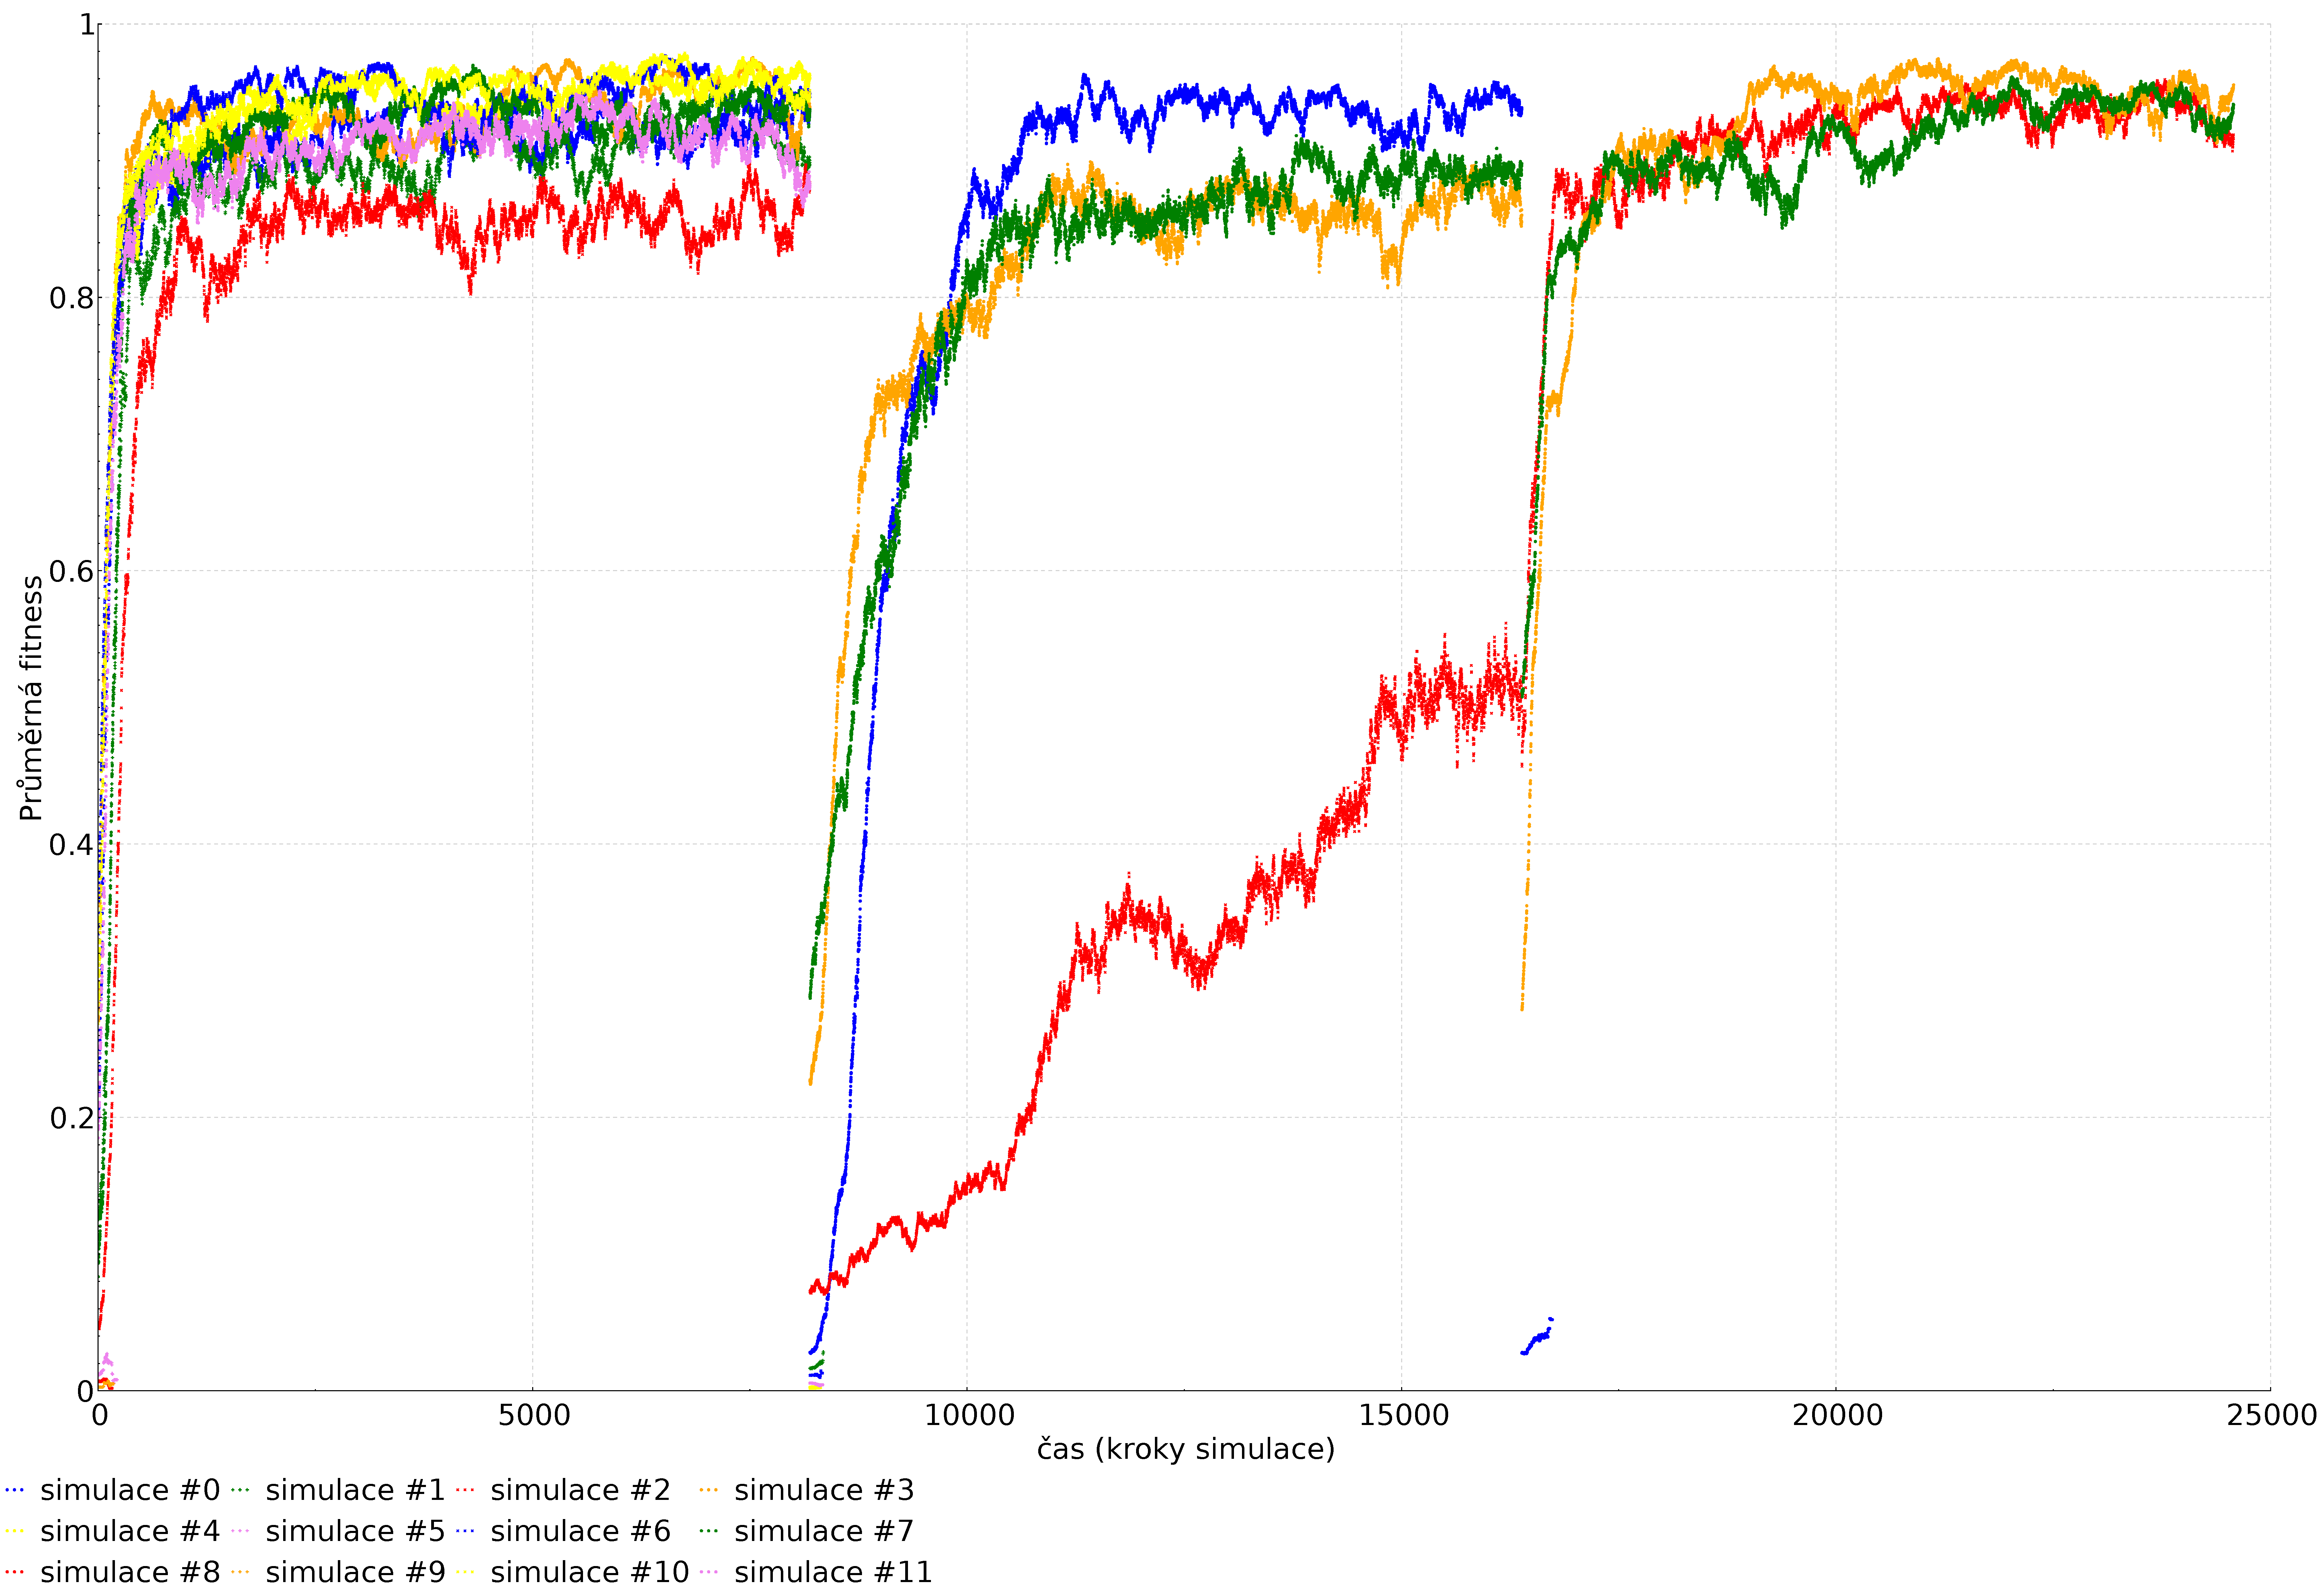
\includegraphics[width=\textwidth]{img/avg_fitness_256_00_00.pdf}

\label{fig:avg_fitness_256_0.0_0.0}

\textit{Podíl alel s negativní dominancí je pravděpodobnost, že nově vzniklá alela bude ovlivňovat fenotyp v opačných
        směrech, pokud bude v lokusu jednou nebo dvakrát. Podíl pleiotropických alel je pravděpodobnost, že nově vzniklá alela
        bude ovlivňovat více složek fenotypu. Rovnovážná velikost populace byla 256 jedinců.}

\end{figure}


\begin{figure}[h]
\caption{Graf vývojů průměrně fitness dvanácti populací pro podíl pleiotropních alel 0.0 a pro podíl negativně
         dominantních alel 0.0}
\centering
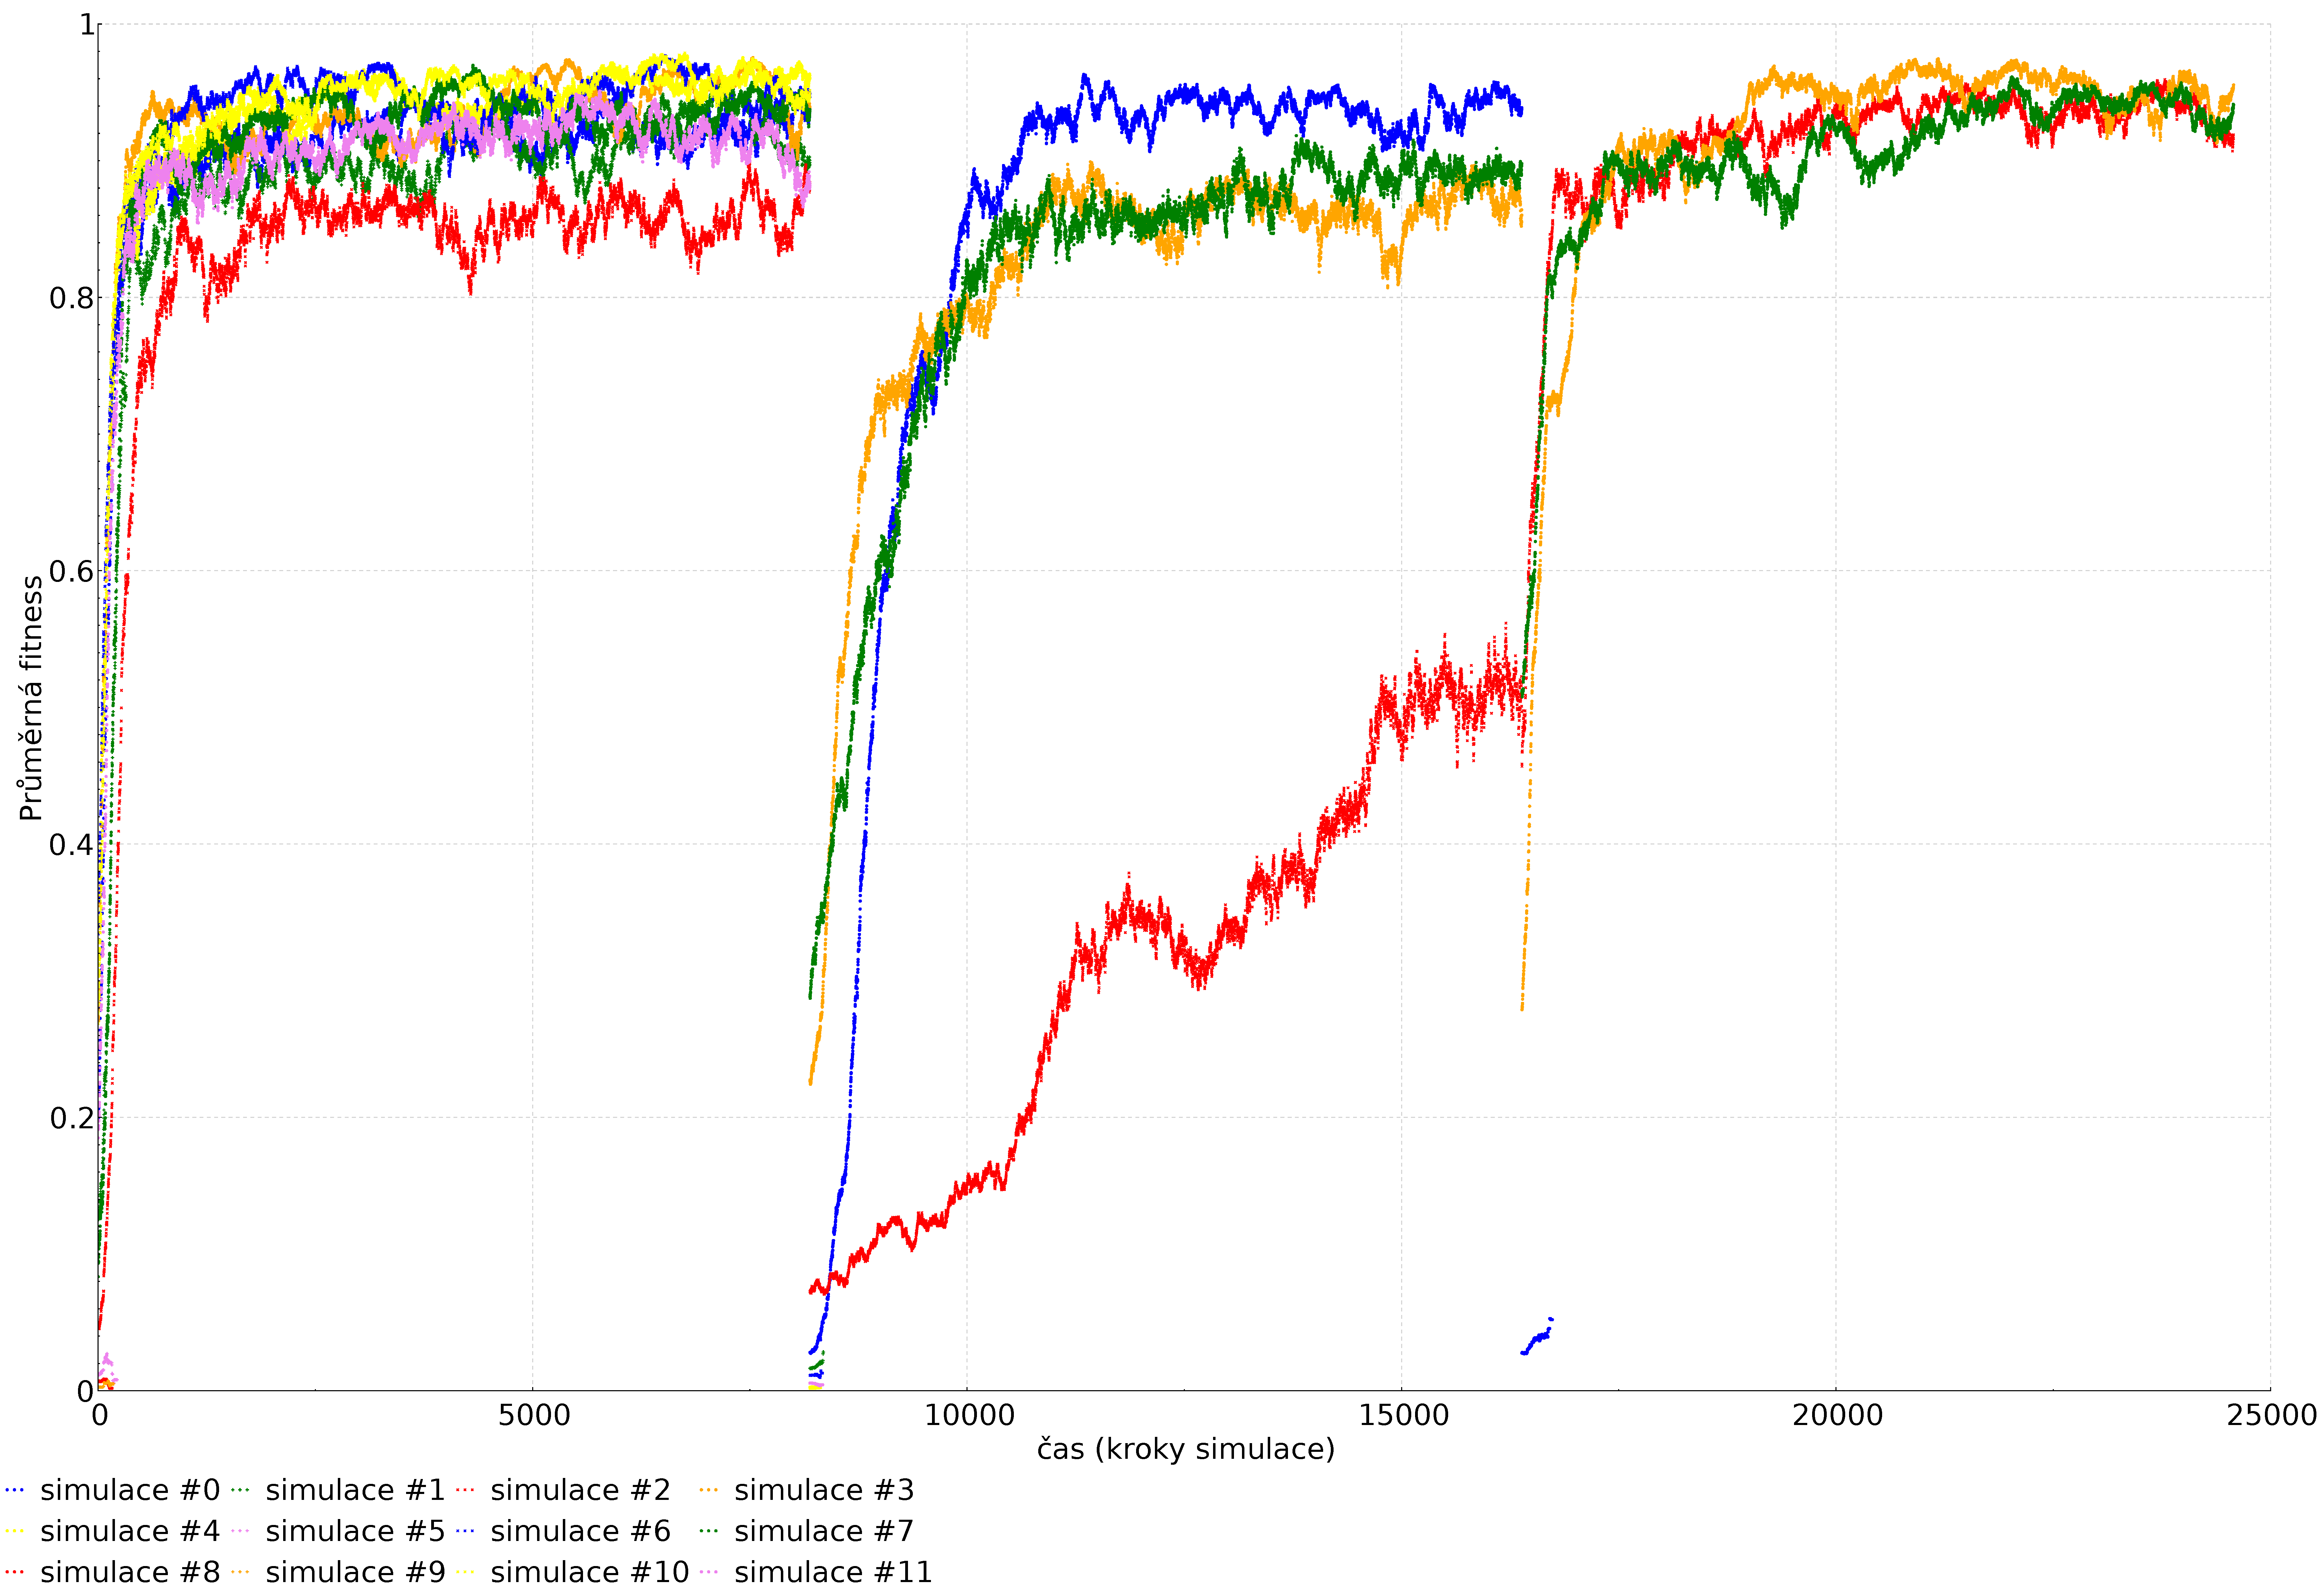
\includegraphics[width=\textwidth]{img/avg_fitness_256_00_00.pdf}

\label{fig:avg_fitness_sssssss256_0.0_0.0}

\textit{Legenda viz legenda k obrázku \ref{fig:avg_fitness_256_0.0_0.0}}

\end{figure}

\begin{figure}[h]
\caption{Graf vývojů průměrně fitness dvanácti populací pro podíl pleiotropních alel 0.0 a pro podíl negativně
         dominantních alel 0.0}
\centering
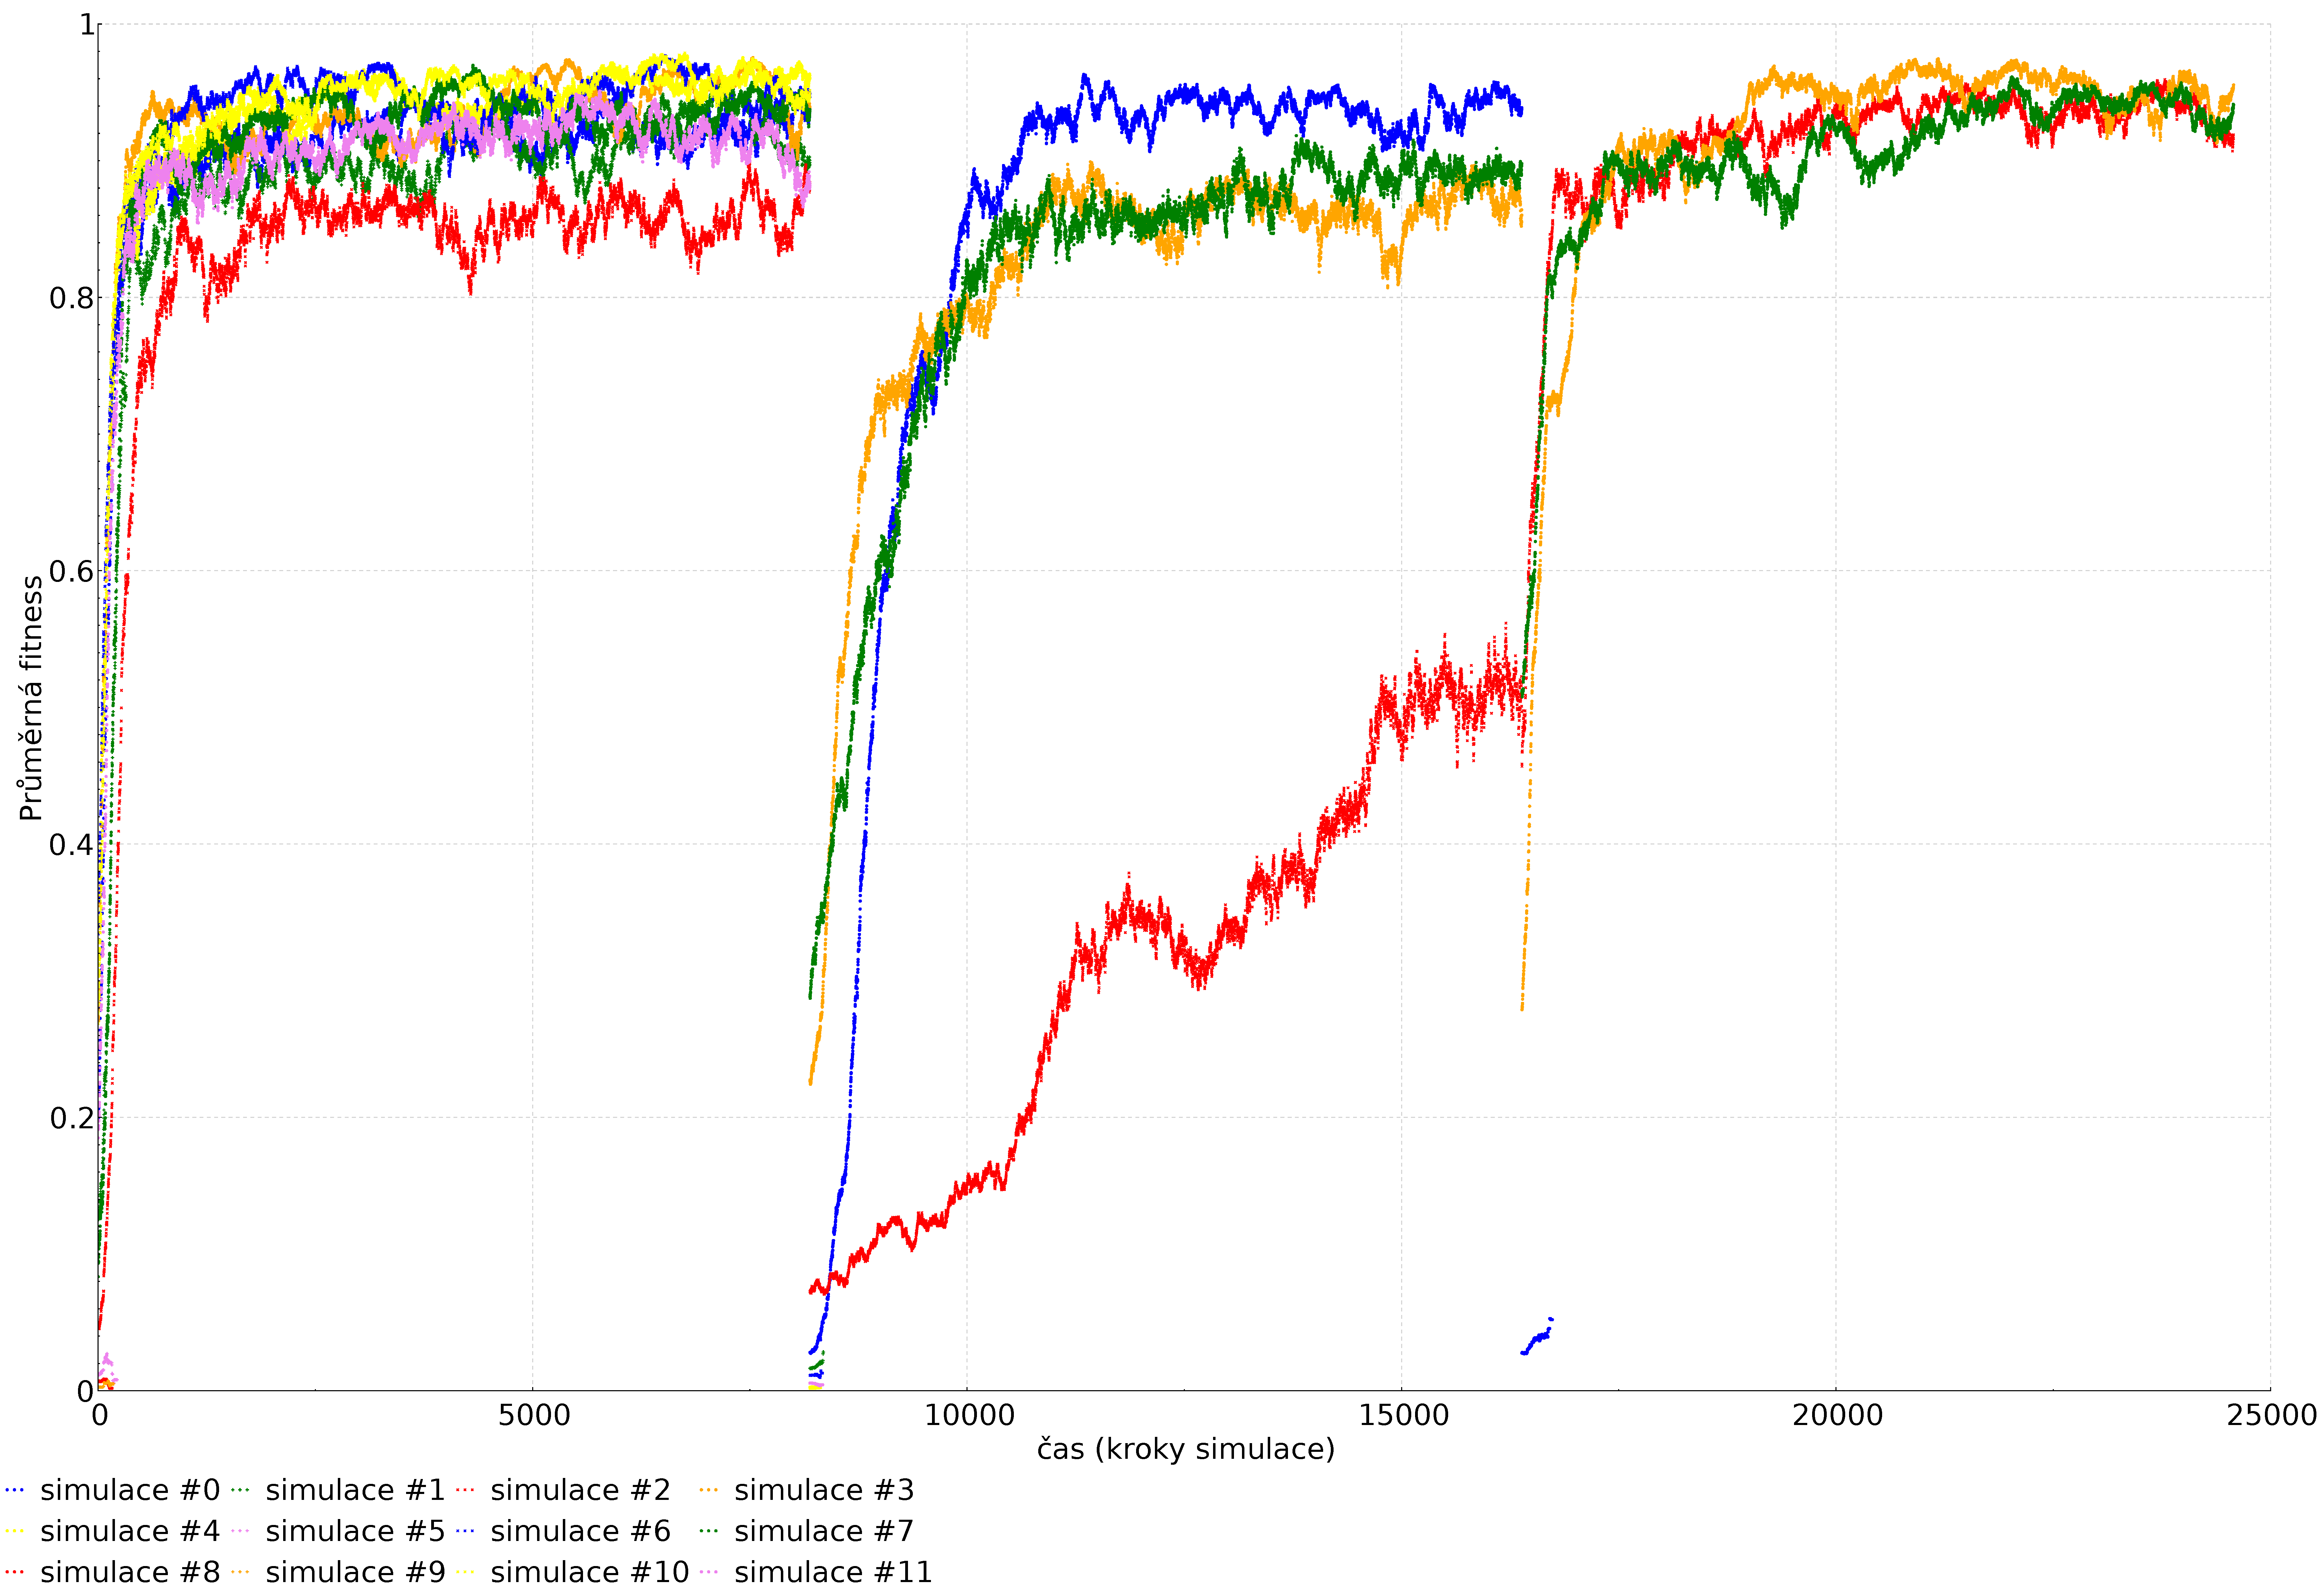
\includegraphics[width=\textwidth]{img/avg_fitness_256_00_00.pdf}

\label{fig:avg_fitness_2sss56_0.0_0.0}

\textit{Legenda viz legenda k obrázku \ref{fig:avg_fitness_256_0.0_0.0}}

\end{figure}